\section{Contributions}\label{contributions}

\subsection{Project Leader (Github reviews \&
merges)}\label{project-leader-github-reviews-merges}

As the project leader, I was responsible for reviewing all pull
requests, ensuring that the code followed the project guidelines, and
merging the code into the main branch. We coordinated through a WhatsApp
group chat and would regularly check in on each other's progress. I
would also signal to the group when code was merged so we could all pull
the latest changes.

Most times, approving and merging was straightforward with no issues,
but there was an interesting challenge when multiple uploads from
different team members overlapped, causing conflicts. This forced us to
learn about stashing and rebasing to the newly updated master branch
before recommitting. The following process was ironed out to ensure a
smooth integration:

\begin{enumerate}
\def\labelenumi{\arabic{enumi}.}
\item
  Stash local (uncommitted) changes

\begin{Shaded}
\begin{Highlighting}[]
   \FunctionTok{git}\NormalTok{ stash}
\end{Highlighting}
\end{Shaded}
\item
  Pull latest changes from master branch

\begin{Shaded}
\begin{Highlighting}[]
   \FunctionTok{git}\NormalTok{ checkout master}
   \FunctionTok{git}\NormalTok{ pull main master}
\end{Highlighting}
\end{Shaded}
\item
  Rebase local changes onto master branch so it starts after the new
  merged code

\begin{Shaded}
\begin{Highlighting}[]
   \FunctionTok{git}\NormalTok{ checkout }\OperatorTok{\textless{}}\NormalTok{fork{-}feature}\OperatorTok{\textgreater{}}\NormalTok{/}\OperatorTok{\textless{}}\NormalTok{fork{-}branch}\OperatorTok{\textgreater{}}
   \FunctionTok{git}\NormalTok{ rebase master}
\end{Highlighting}
\end{Shaded}
\item
  Resolve any conflicts \& re-apply stashed changes

\begin{Shaded}
\begin{Highlighting}[]
   \FunctionTok{git}\NormalTok{ stash pop}
\end{Highlighting}
\end{Shaded}
\item
  Commit and push (using \texttt{-\/-force} parameter due to rebase)

\begin{Shaded}
\begin{Highlighting}[]
   \FunctionTok{git}\NormalTok{ push }\OperatorTok{\textless{}}\NormalTok{fork{-}remote}\OperatorTok{\textgreater{}} \OperatorTok{\textless{}}\NormalTok{fork{-}branch}\OperatorTok{\textgreater{}}\NormalTok{ {-}{-}force}
\end{Highlighting}
\end{Shaded}
\end{enumerate}

\subsection{Makefile}\label{makefile}

As the project evolved, so did the Makefile. Here are some of the
features we implemented:

Starting off, there are few main variables that control the compilation
process.

\begin{Shaded}
\begin{Highlighting}[]
\DataTypeTok{FC}       \CharTok{=}\StringTok{ gfortran}
\DataTypeTok{FFLAGS}   \CharTok{=}\StringTok{ {-}O2 {-}Wall {-}Wextra}
\DataTypeTok{OBJ\_DIR}  \CharTok{=}\StringTok{ ../bin}
\DataTypeTok{EXE}      \CharTok{=}\StringTok{ }\CharTok{$(}\DataTypeTok{OBJ\_DIR}\CharTok{)}\StringTok{/main\_serial.x}
\DataTypeTok{LIB\_OBJ}  \CharTok{=}\StringTok{ }\CharTok{$(}\DataTypeTok{OBJ\_DIR}\CharTok{)}\StringTok{/parameters.o }\CharTok{\textbackslash{}}
\StringTok{           }\CharTok{$(}\DataTypeTok{OBJ\_DIR}\CharTok{)}\StringTok{/io.o }\CharTok{\textbackslash{}}
\StringTok{           ...}
\DataTypeTok{MAIN\_OBJ} \CharTok{=}\StringTok{ }\CharTok{$(}\DataTypeTok{OBJ\_DIR}\CharTok{)}\StringTok{/main\_serial.o}

\DataTypeTok{NP}          \CharTok{?=}\StringTok{ 4}
\DataTypeTok{OMP\_THREADS} \CharTok{?=}\StringTok{ 2}
\end{Highlighting}
\end{Shaded}

\begin{itemize}
\tightlist
\item
  \texttt{FC}: Stands for ``Fortran Compiler''. We tell it to use
  gfortran.
\item
  \texttt{FFLAGS}: These are the compiler flags. \texttt{-O2} is the
  optimization schema, and \texttt{-Wall\ -Wextra} enables warnings.
\item
  \texttt{OBJ\_DIR} \& \texttt{EXE}: Defines the compiled binaries
  directory and the name of the final executable.
\item
  \texttt{LIB\_OBJ} \& \texttt{MAIN\_OBJ}: Defines the object files for
  the library and the main program.
\item
  \texttt{NP} \& \texttt{OMP\_THREADS}: Defines the number of processes
  (MPI) and threads (openMP) to use for the parallel version of the
  program. The default values are set to 4 and 2, respectively, but they
  can be overridden by setting them when compiling in the command line
  (e.g., \texttt{make\ run\_parallel\ NP=7\ OMP\_THREADS=3}).
\end{itemize}

In order to encompass both the serial and parallel versions of the
program, we perform a check on the make command for the word
\texttt{parallel}. If found, we search the system to ensure the user
enviroment has the necessary MPI and OpenMP libraries installed. If not,
we print an error message and exit. If they are installed, we overwrite
the compiler and add the MPI and OpenMP flags to the \texttt{FFLAGS}
variable.

\begin{Shaded}
\begin{Highlighting}[]
\ControlFlowTok{ifneq}\NormalTok{ (,}\CharTok{$(}\KeywordTok{findstring}\StringTok{ parallel}\KeywordTok{,}\CharTok{$(}\DataTypeTok{MAKECMDGOALS}\CharTok{))}\NormalTok{)}
  \CommentTok{\# MPI Compiler Wrapper Verification}
  \DataTypeTok{MPI\_BIN} \CharTok{:=}\StringTok{ }\CharTok{$(}\KeywordTok{shell}\StringTok{ command {-}v mpif90 2\textgreater{}/dev/null}\CharTok{)}
  \ControlFlowTok{ifeq}\NormalTok{ (}\CharTok{$(}\KeywordTok{strip}\StringTok{ }\CharTok{$(}\DataTypeTok{MPI\_BIN}\CharTok{))}\NormalTok{,)}
    \CharTok{$(}\KeywordTok{error}\StringTok{ "MPI Compiler is required but \textquotesingle{}mpif90\textquotesingle{} was not found! Please install it (e.g. \textquotesingle{}sudo apt install openmpi{-}bin\textquotesingle{})"}\CharTok{)}
  \ControlFlowTok{endif}
  \CommentTok{\# Overwrite Compiler for MPI parallelization flag linking}
  \DataTypeTok{FC} \CharTok{=}\StringTok{ mpif90}
\NormalTok{  ...}
\end{Highlighting}
\end{Shaded}

Instead of writing a rule for every single \texttt{.f90} file, we use a
pattern rule (using \texttt{\%}).

\begin{Shaded}
\begin{Highlighting}[]
\DecValTok{$(OBJ\_DIR)/\%.o:}\DataTypeTok{ lib/\%.f90}
\ErrorTok{    }\CharTok{@}\FunctionTok{mkdir {-}p }\CharTok{$(}\DataTypeTok{OBJ\_DIR}\CharTok{)}
    \CharTok{$(}\DataTypeTok{FC}\CharTok{)} \CharTok{$(}\DataTypeTok{FFLAGS}\CharTok{)}\NormalTok{ {-}J}\CharTok{$(}\DataTypeTok{OBJ\_DIR}\CharTok{)}\NormalTok{ {-}I}\CharTok{$(}\DataTypeTok{OBJ\_DIR}\CharTok{)}\NormalTok{ {-}c }\CharTok{$\textless{}}\NormalTok{ {-}o }\CharTok{$@}
\end{Highlighting}
\end{Shaded}

\begin{itemize}
\tightlist
\item
  It says: ``To make any \texttt{.o} file in the object directory
  (\texttt{bin/}) from a matching \texttt{.f90} file in \texttt{lib/},
  run this command.''
\item
  \texttt{-c\ \$\textless{}}: Compiles the ``first dependency''
  (\texttt{\$\textless{}}, which is the \texttt{.f90} file) without
  linking (because that's done in the \texttt{\$(EXE)} target).
\item
  \texttt{-J\$(OBJ\_DIR)\ -I\$(OBJ\_DIR)}: Tells Fortran to put module
  \texttt{.mod} files in the \texttt{bin/} folder.
\end{itemize}

The following is an example of the \texttt{all} target (serial version
of the program) with its executable structure, which we then follow up
with the explicit dependencies to create the \texttt{.o} files for the
library modules and the main program

\begin{Shaded}
\begin{Highlighting}[]
\DecValTok{all:}\DataTypeTok{ }\CharTok{$(}\DataTypeTok{EXE}\CharTok{)}

\DecValTok{$(EXE):}\DataTypeTok{ }\CharTok{$(}\DataTypeTok{LIB\_OBJ}\CharTok{)}\DataTypeTok{ }\CharTok{$(}\DataTypeTok{MAIN\_OBJ}\CharTok{)}
\ErrorTok{    }\CharTok{@}\FunctionTok{mkdir {-}p }\CharTok{$(}\DataTypeTok{OBJ\_DIR}\CharTok{)}
    \CharTok{$(}\DataTypeTok{FC}\CharTok{)} \CharTok{$(}\DataTypeTok{FFLAGS}\CharTok{)}\NormalTok{ {-}o }\CharTok{$@} \CharTok{$(}\DataTypeTok{LIB\_OBJ}\CharTok{)} \CharTok{$(}\DataTypeTok{MAIN\_OBJ}\CharTok{)}

\DecValTok{$(OBJ\_DIR)/energy.o:}\DataTypeTok{ lib/energy.f90 }\CharTok{\textbackslash{}}
\DataTypeTok{                     }\CharTok{$(}\DataTypeTok{OBJ\_DIR}\CharTok{)}\DataTypeTok{/parameters.o}
\NormalTok{...}

\DecValTok{$(OBJ\_DIR)/main\_serial.o:}\DataTypeTok{ main\_serial.f90 }\CharTok{$(}\DataTypeTok{LIB\_OBJ}\CharTok{)}
\ErrorTok{    }\CharTok{@}\FunctionTok{mkdir {-}p }\CharTok{$(}\DataTypeTok{OBJ\_DIR}\CharTok{)}
    \CharTok{$(}\DataTypeTok{FC}\CharTok{)} \CharTok{$(}\DataTypeTok{FFLAGS}\CharTok{)}\NormalTok{ {-}J}\CharTok{$(}\DataTypeTok{OBJ\_DIR}\CharTok{)}\NormalTok{ {-}I}\CharTok{$(}\DataTypeTok{OBJ\_DIR}\CharTok{)}\NormalTok{ {-}c }\CharTok{$\textless{}}\NormalTok{ {-}o }\CharTok{$@}
\end{Highlighting}
\end{Shaded}

\begin{itemize}
\tightlist
\item
  \texttt{all}: This is the default target that needs \texttt{\$(EXE)}
  to exist.
\item
  \texttt{\$(EXE)}: To build the final executable, it needs all the .o
  files from the \texttt{../bin} folder, which it makes sure exists
  (\texttt{mkdir\ -p}), and then links them all together using
  \texttt{gfortran} or \texttt{mpif90} to output (\texttt{-o\ \$@}) the
  final program.

  \begin{itemize}
  \tightlist
  \item
    \textbf{Note}: The \texttt{@} symbol is used 2 different ways here:

    \begin{enumerate}
    \def\labelenumi{\arabic{enumi}.}
    \tightlist
    \item
      Before the \texttt{mkdir} command to suppress being printed to the
      terminal.
    \item
      As an automatic variable representing the target name
      (\texttt{\$(EXE)} in this case).
    \end{enumerate}
  \end{itemize}
\end{itemize}

Last, we declare the shortcut commands as \texttt{.PHONY} targets to
prevent conflicts with files that may have the same name as a target.

\begin{Shaded}
\begin{Highlighting}[]
\OtherTok{.PHONY:}\DataTypeTok{ all clean run figures pipeline}

\DecValTok{run:}\DataTypeTok{ all}
\ErrorTok{    }\CharTok{@}\FunctionTok{mkdir {-}p ../results}
    \CharTok{$(}\DataTypeTok{EXE}\CharTok{)}

\DecValTok{figures:}
\ErrorTok{    }\NormalTok{python lib/plot\_results.py}

\DecValTok{clean:}\DataTypeTok{ }
\ErrorTok{    }\NormalTok{rm {-}rf }\CharTok{$(}\DataTypeTok{OBJ\_DIR}\CharTok{)}\NormalTok{/*.o }\CharTok{$(}\DataTypeTok{OBJ\_DIR}\CharTok{)}\NormalTok{/*.mod }\CharTok{$(}\DataTypeTok{EXE}\CharTok{)}

\DecValTok{pipeline:}
\ErrorTok{    }\CharTok{$(}\DataTypeTok{MAKE}\CharTok{)}\NormalTok{ run}
    \CharTok{$(}\DataTypeTok{MAKE}\CharTok{)}\NormalTok{ figures}
\end{Highlighting}
\end{Shaded}

\begin{itemize}
\tightlist
\item
  This enables the following compile-time shortcuts:

  \begin{itemize}
  \tightlist
  \item
    \texttt{make\ run}: Automatically builds the code (\texttt{all}) and
    then executes it.
  \item
    \texttt{make\ figures}: Envokes python to generate the plots from
    the \texttt{../results} folder.
  \item
    \texttt{make\ clean}: Acts like a reset button, deleting all
    compiled files to start fresh.
  \item
    \texttt{make\ pipeline}: A neat wrapper we built to run the code and
    generate the python plots back-to-back.
  \end{itemize}
\end{itemize}

\subsection{Main - Serial}\label{main---serial}

Since the initial code submission, we have updated the serial version of
our file \texttt{main\_serial\_equil.f90} to incorporate an
equilibration check based on the Geweke equilibration diagnostic
(Geweke, J. 1992). Specifically designed for Markov Chain Monte Carlo
simulations, this technique allows us to separate the simulation into
equilibration and production phases during runtime as opposed to
analyzing the results afterwards. It also allows us to identify and save
an equilibrated geometry which can then be used to save time by
bypassing the initial phase.

The simulation begins by reading in the configurations from
\texttt{input.dat} and building the starting coordinates. If these are
not overwritten by a previously saved equilibration .xyz file, the
program will initialized and enter \textbf{Phase 1: Equilibration}.

\begin{Shaded}
\begin{Highlighting}[]
  \KeywordTok{do} \KeywordTok{while}\NormalTok{ (}\OperatorTok{.not.}\NormalTok{ is\_equilibrated)}
\NormalTok{    istep }\KeywordTok{=}\NormalTok{ istep }\KeywordTok{+} \DecValTok{1}

    \CommentTok{! Annealing:}
    \KeywordTok{if}\NormalTok{ (istep }\OperatorTok{\textless{}=}\NormalTok{ n\_steps) }\KeywordTok{then}
\NormalTok{      T }\KeywordTok{=}\NormalTok{ T\_ini }\KeywordTok{{-}}\NormalTok{ dT }\KeywordTok{*} \BuiltInTok{dble}\NormalTok{(istep }\KeywordTok{{-}} \DecValTok{1}\NormalTok{)}
    \KeywordTok{else}
\NormalTok{      T }\KeywordTok{=}\NormalTok{ T\_fin}
    \KeywordTok{end if}
    
    \CommentTok{! Monte Carlo Step}
    \KeywordTok{call}\NormalTok{ mc\_step(n\_carbons, n\_atoms, coords, symbols, explicit\_h, }\KeywordTok{\&}
\NormalTok{                 beta, max\_delta, E\_total, E\_lj, E\_tors, accepted\_step)}
    
    \KeywordTok{if}\NormalTok{ (accepted\_step) total\_accepted }\KeywordTok{=}\NormalTok{ total\_accepted }\KeywordTok{+} \DecValTok{1}

    \CommentTok{! Output periodically}
    \KeywordTok{if}\NormalTok{ (}\BuiltInTok{mod}\NormalTok{(istep, print\_interval) }\OperatorTok{==} \DecValTok{0} \OperatorTok{.or.}\NormalTok{ istep }\OperatorTok{==} \DecValTok{1}\NormalTok{) }\KeywordTok{then}
      \CommentTok{! Energies}
      \FunctionTok{write(}\NormalTok{u\_ener, }\StringTok{\textquotesingle{}(I10, 3F15.4)\textquotesingle{}}\FunctionTok{)}\NormalTok{ istep, E\_total, E\_lj, E\_tors}

      \CommentTok{! Observables}
\NormalTok{      rg2 }\KeywordTok{=}\NormalTok{ compute\_rg(n\_carbons, coords)}
\NormalTok{      ree2 }\KeywordTok{=}\NormalTok{ compute\_end\_to\_}\KeywordTok{end}\NormalTok{(n\_carbons, coords)}
      \FunctionTok{write(}\NormalTok{u\_obs, }\StringTok{\textquotesingle{}(I10, 2F15.4)\textquotesingle{}}\FunctionTok{)}\NormalTok{ istep, }\BuiltInTok{sqrt}\NormalTok{(rg2), }\BuiltInTok{sqrt}\NormalTok{(ree2)}
\NormalTok{      ...}
\end{Highlighting}
\end{Shaded}

\begin{itemize}
\tightlist
\item
  \texttt{do\ while\ (.not.\ is\_equilibrated)}: Replaces traditional
  hard-coded burn-in periods with a dynamic loop that stays alive until
  equilibration is met.
\item
  \texttt{T\ =\ T\_ini\ -\ dT\ *\ dble(istep\ -\ 1)}: We had originally
  discussed introducing simulated annealing to help the simulation
  escape local minima, however the project instructions say to assume a
  fixed temperature. This portion of the code was left in case we wanted
  to set T\_ini \& T\_fin to different values.
\item
  \texttt{call\ mc\_step(...)}: Subroutine to perform a single Monte
  Carlo step.
\item
  We control when to compute \& store the observables (energy, torsion,
  trajectory, etc) based on the \texttt{print\_interval} variable.
\end{itemize}

\section{--------- MANEL REVIEW NEEDED
---------}\label{manel-review-needed}

As stated above we use the Geweke equilibration diagnostic for a dynamic
determination of reaching equilibrium. To prevent false positives due to
auto-correlation between adjacent MC steps, we evaluate the system
periodically:

\begin{Shaded}
\begin{Highlighting}[]
    \CommentTok{! {-}{-}{-} Geweke Check {-}{-}{-}}
    \KeywordTok{if}\NormalTok{ (}\BuiltInTok{mod}\NormalTok{(istep, geweke\_sample\_interval) }\OperatorTok{==} \DecValTok{0}\NormalTok{) }\KeywordTok{then}
      
\NormalTok{      gbuf\_count }\KeywordTok{=}\NormalTok{ gbuf\_count }\KeywordTok{+} \DecValTok{1}
      \KeywordTok{if}\NormalTok{ (gbuf\_count }\OperatorTok{\textless{}=}\NormalTok{ n\_geweke) }\KeywordTok{then}
\NormalTok{        gbuf\_E(gbuf\_count) }\KeywordTok{=}\NormalTok{ E\_total}
\NormalTok{        gbuf\_Rg(gbuf\_count) }\KeywordTok{=}\NormalTok{ rg2}
      \KeywordTok{else}
        \CommentTok{! ... (shift buffer and add new state) ...}
      \KeywordTok{end if}
      
      \KeywordTok{if}\NormalTok{ (gbuf\_count }\OperatorTok{\textgreater{}=}\NormalTok{ n\_geweke }\OperatorTok{.and.} \BuiltInTok{mod}\NormalTok{(gbuf\_count, eval\_freq) }\OperatorTok{==} \DecValTok{0}\NormalTok{) }\CommentTok{then}
        \CommentTok{! ... (calculate standard errors and Z{-}scores) ...}
        \KeywordTok{if}\NormalTok{ (z\_E }\OperatorTok{\textless{}}\NormalTok{ z\_crit) }\KeywordTok{then}
            \CommentTok{! ... }
\NormalTok{            is\_equilibrated }\KeywordTok{=} \ConstantTok{.true.}
\NormalTok{      ...}
\end{Highlighting}
\end{Shaded}

\begin{itemize}
\tightlist
\item
  \texttt{mod(istep,\ geweke\_sample\_interval)\ ==\ 0}: Enforces
  periodic sampling (e.g., every 10,000 steps) so the data points
  entering the convergence test are truly statistically independent.
\item
  \texttt{gbuf\_E} \& \texttt{gbuf\_Rg}: Sliding window arrays of size
  \texttt{n\_geweke} (300) that hold the recent energy and Radius of
  Gyration states respectively.
\item
  \texttt{z\_E\ \textless{}\ z\_crit}: Evaluates the \(Z\)-score
  comparing the means of the first 10\% and last 50\% of the buffer. If
  it falls below the critical threshold (\(1.96\)), the system is
  flagged as structurally stable (\texttt{is\_equilibrated\ =\ .true.}).
\end{itemize}

Once equilibrium is reached, all Phase 1 files are closed and the
program transitions seamlessly into \textbf{Phase 2: Production},
resetting the clock and creating new tracking files.

\begin{Shaded}
\begin{Highlighting}[]
  \CommentTok{! ======================================================}
  \CommentTok{! PHASE 2: PRODUCTION}
  \CommentTok{! ======================================================}
  
  \KeywordTok{call}\NormalTok{ cpu\_time(cpu\_start)}
  \KeywordTok{do}\NormalTok{ istep }\KeywordTok{=} \DecValTok{1}\NormalTok{, n\_steps}

    \KeywordTok{call}\NormalTok{ mc\_step(n\_carbons, n\_atoms, coords, symbols, explicit\_h, }\KeywordTok{\&}
\NormalTok{                 beta, max\_delta, E\_total, E\_lj, E\_tors, accepted\_step)}
\NormalTok{  ...}
\end{Highlighting}
\end{Shaded}

\begin{itemize}
\tightlist
\item
  \texttt{call\ cpu\_time(cpu\_start)}: We separate the 2 phases' timers
  to assist in benchmarking as there is the ability to preload an
  equilibrated geometry and go straight into production.
\item
  \texttt{n\_steps}: Benchmarking the benefits of parallelization is
  also helped by ensuring production runs have the same number of MCS
  performed. This can be controlled from the \texttt{input.dat} file
  settings.
\end{itemize}

\subsection{Visualization}\label{visualization}

The visualization of our results is handled by
\texttt{plot\_results.py}. It starts by reading the \texttt{input.dat}
file to determine whether the simulation was run using explicit
hydrogens so it knows which theoretical potential to compare against.

\section{--------- Itxaso Review Needed
-------------}\label{itxaso-review-needed--}

Before plotting the torsion angles, the script conducts a statistical
analysis to detect when the Monte Carlo simulation reaches thermodynamic
equilibrium, so it can discard the burn-in period.

\begin{Shaded}
\begin{Highlighting}[]
\KeywordTok{def}\NormalTok{ detect\_equilibration(x):}
    \CommentTok{\# Chodera (2016) method to find optimal equilibration index (t0)}
\NormalTok{    n }\OperatorTok{=} \BuiltInTok{len}\NormalTok{(x)}
\NormalTok{    best\_neff }\OperatorTok{=} \FloatTok{0.0}
\NormalTok{    best\_t0 }\OperatorTok{=} \DecValTok{0}
    
\NormalTok{    candidates }\OperatorTok{=}\NormalTok{ np.unique(np.linspace(}\DecValTok{0}\NormalTok{, }\BuiltInTok{int}\NormalTok{(n }\OperatorTok{*} \FloatTok{0.9}\NormalTok{), }\BuiltInTok{min}\NormalTok{(}\DecValTok{200}\NormalTok{, n)).astype(}\BuiltInTok{int}\NormalTok{))}
    \ControlFlowTok{for}\NormalTok{ t0 }\KeywordTok{in}\NormalTok{ candidates:}
\NormalTok{        sub }\OperatorTok{=}\NormalTok{ x[t0:]}
\NormalTok{        \_, g }\OperatorTok{=}\NormalTok{ integrated\_autocorr\_time(sub)}
\NormalTok{        neff }\OperatorTok{=}\NormalTok{ (n }\OperatorTok{{-}}\NormalTok{ t0) }\OperatorTok{/}\NormalTok{ g}
        \ControlFlowTok{if}\NormalTok{ neff }\OperatorTok{\textgreater{}}\NormalTok{ best\_neff:}
\NormalTok{            best\_neff, best\_t0 }\OperatorTok{=}\NormalTok{ neff, t0}
            
    \ControlFlowTok{return}\NormalTok{ best\_t0}
\end{Highlighting}
\end{Shaded}

\begin{itemize}
\tightlist
\item
  \texttt{integrated\_autocorr\_time(sub)}: Calculates the statistical
  inefficiency (\(g\)) and the integrated autocorrelation time
  (\(\tau_{int}\)) of the dataset using Fast Fourier Transforms (FFT).
\item
  \texttt{neff\ =\ (n\ -\ t0)\ /\ g}: Estimates the number of
  effectively uncorrelated samples.
\item
  \texttt{best\_t0}: The algorithm sweeps through candidate discard
  points and selects the index t0 that maximizes the effective sample
  size, marking the end of the equilibration phase.
\end{itemize}

\section{------------------------------------------------}\label{section}

Then, there are 3 defined functions for each of the plots using
matplotlib: * \texttt{plot\_energies}: Plots the total energy, LJ
energy, and torsion energy against the MC steps. *
\texttt{plot\_observables}: Plots the radius of gyration and end-to-end
distance against the MC steps. * \texttt{plot\_torsions}: Plots the
torsion angles against the MC steps and compares them to the theoretical
potential.

Finally, the script moves on to generating the actual .pdf plots using
matplotlib. The most complex of these is the torsion distribution plot,
which overlays our histogram data against the theoretical TraPPE
potentials.

\begin{Shaded}
\begin{Highlighting}[]
\KeywordTok{def}\NormalTok{ plot\_torsions(tors\_file, energy\_file, explicit\_h}\OperatorTok{=}\VariableTok{True}\NormalTok{):}
    \ControlFlowTok{if} \KeywordTok{not}\NormalTok{ explicit\_h:}
\NormalTok{        c1, c2, c3 }\OperatorTok{=} \FloatTok{0.705}\NormalTok{, }\OperatorTok{{-}}\FloatTok{0.135}\NormalTok{, }\FloatTok{1.572}
    \ControlFlowTok{else}\NormalTok{:}
\NormalTok{        c1, c2, c3 }\OperatorTok{=} \FloatTok{0.8700}\NormalTok{, }\OperatorTok{{-}}\FloatTok{0.0785}\NormalTok{, }\FloatTok{1.5075}
    \KeywordTok{def}\NormalTok{ torsion\_potential(phi):}
        \ControlFlowTok{return}\NormalTok{ (c1 }\OperatorTok{*}\NormalTok{ (}\FloatTok{1.0} \OperatorTok{+}\NormalTok{ np.cos(phi))}
              \OperatorTok{+}\NormalTok{ c2 }\OperatorTok{*}\NormalTok{ (}\FloatTok{1.0} \OperatorTok{{-}}\NormalTok{ np.cos(}\FloatTok{2.0} \OperatorTok{*}\NormalTok{ phi))}
              \OperatorTok{+}\NormalTok{ c3 }\OperatorTok{*}\NormalTok{ (}\FloatTok{1.0} \OperatorTok{+}\NormalTok{ np.cos(}\FloatTok{3.0} \OperatorTok{*}\NormalTok{ phi)))}
\end{Highlighting}
\end{Shaded}

\begin{itemize}
\tightlist
\item
  \texttt{explicit\_h}: The boolean passed from our parser function.
\item
  \texttt{c1,\ c2,\ c3}: The TraPPE-UA United Atom coefficients, or the
  OPLS-AA Effective Backbone coefficients, loaded depending on the
  simulation type.
\item
  \texttt{torsion\_potential(phi)}: Returns the theoretical energy (in
  kcal/mol) for any given dihedral angle (\(\phi\)) using trigonometric
  identities, which is then overlaid on the secondary Y-axis spanning
  across the histograms.
\end{itemize}

\subsection{Parallelization - Ensemble
Averaging}\label{parallelization---ensemble-averaging}

Moving to an Orchestrator-Worker (Star) topology helped with the
transition of the serial environment to a dynamically balanced parallel
framework with OpenMPI. It achieves maximum CPU utilization by ensuring
free workers are constantly assigned tasks until the simulation is
complete.

Although this architechure adds overhead by requiring a single core to
abstain from participating in the simulation's calculations, the
orchestrator node performs the administrative tasks such as the initial
file reading as well as organizing and distributing the workload. This
relies upon tags being sent between the nodes to coordinate the
simulation.

\begin{Shaded}
\begin{Highlighting}[]
  \CommentTok{! MPI Tags}
  \DataTypeTok{integer}\NormalTok{, }\DataTypeTok{parameter} \DataTypeTok{::}\NormalTok{ TAG\_REQUEST\_WORK }\KeywordTok{=} \DecValTok{1}
  \DataTypeTok{integer}\NormalTok{, }\DataTypeTok{parameter} \DataTypeTok{::}\NormalTok{ TAG\_DO\_EQUIL     }\KeywordTok{=} \DecValTok{2}
  \DataTypeTok{integer}\NormalTok{, }\DataTypeTok{parameter} \DataTypeTok{::}\NormalTok{ TAG\_DO\_PROD      }\KeywordTok{=} \DecValTok{3}
  \DataTypeTok{integer}\NormalTok{, }\DataTypeTok{parameter} \DataTypeTok{::}\NormalTok{ TAG\_WAIT         }\KeywordTok{=} \DecValTok{4}
  \DataTypeTok{integer}\NormalTok{, }\DataTypeTok{parameter} \DataTypeTok{::}\NormalTok{ TAG\_DIE          }\KeywordTok{=} \DecValTok{5}
  \DataTypeTok{integer}\NormalTok{, }\DataTypeTok{parameter} \DataTypeTok{::}\NormalTok{ TAG\_EQUIL\_DONE   }\KeywordTok{=} \DecValTok{6}
  \DataTypeTok{integer}\NormalTok{, }\DataTypeTok{parameter} \DataTypeTok{::}\NormalTok{ TAG\_PROD\_DONE    }\KeywordTok{=} \DecValTok{7}
\end{Highlighting}
\end{Shaded}

First, the simulation is cleanly segregated into phases where the
\textbf{Orchestrator Node} acts as a central dispatcher:

\begin{Shaded}
\begin{Highlighting}[]
      \KeywordTok{do} \KeywordTok{while}\NormalTok{ (completed\_prods }\OperatorTok{\textless{}} \FunctionTok{size}\NormalTok{(prod\_queue))}
         \CommentTok{! Wait for any worker to finish its task and ask for more}
         \KeywordTok{call}\NormalTok{ MPI\_Recv(msg, }\DecValTok{1}\NormalTok{, MPI\_INTEGER, MPI\_ANY\_SOURCE, MPI\_ANY\_TAG,}\CommentTok{ MPI\_COMM\_WORLD, status, ierr)}
\NormalTok{         sender }\KeywordTok{=}\NormalTok{ status(MPI\_SOURCE)}
\NormalTok{         tag\_recvd }\KeywordTok{=}\NormalTok{ status(MPI\_TAG)}
\end{Highlighting}
\end{Shaded}

\begin{itemize}
\tightlist
\item
  \texttt{MPI\_Recv}: The orchestrator lies in wait for any incoming
  communication from the worker nodes.
\item
  \texttt{MPI\_ANY\_SOURCE}: Instead of statically assigning jobs to
  specific processors up-front, the orchestrator listens to the
  \emph{entire pool} of available cores. As soon as a worker node
  finishes its current 1-million-step job, it pings the orchestrator,
  which instantly deploys the next job from the queue directly to that
  specific idle worker, ensuring optimal resource utilization.
\item
  \textbf{Staged Execution}: By cleanly separating the logic phases, the
  orchestrator refuses to load the 10 production jobs into the queue
  until the prerequisite equilibration run officially finishes. The
  moment equilibration is met, jobs pop into the queue and cores are
  reused instantly, guaranteeing no resources are ever permanently
  ``blocked'' waiting in idle lines.
\end{itemize}

Once a worker has sent an incoming communication signal back to the
orchestrator, the orchestrator checks the tag and executes the
appropriate logic:

\begin{Shaded}
\begin{Highlighting}[]
         \KeywordTok{if}\NormalTok{ (tag\_recvd }\OperatorTok{==}\NormalTok{ TAG\_EQUIL\_DONE) }\KeywordTok{then}
           \CommentTok{! ... (Orchestrator caches the equilibrated .xyz coordinates and unlocks the production queue)}
         \KeywordTok{else if}\NormalTok{ (tag\_recvd }\OperatorTok{==}\NormalTok{ TAG\_PROD\_DONE) }\KeywordTok{then} 
           \CommentTok{! ... (Orchestrator tallies the completed production run)}
         \KeywordTok{end if}

         \CommentTok{! If jobs remain in the queue, immediately deploy the next one to the \textquotesingle{}sender\textquotesingle{}}
         \KeywordTok{if}\NormalTok{ (jobs\_assigned }\OperatorTok{\textless{}} \FunctionTok{size}\NormalTok{(prod\_queue)) }\KeywordTok{then}
            \KeywordTok{call}\NormalTok{ MPI\_Send(TAG\_DO\_PROD, }\DecValTok{1}\NormalTok{, MPI\_INTEGER, sender, TAG\_DO\_PROD, MPI\_COMM\_WORLD, ierr)}
\end{Highlighting}
\end{Shaded}

\begin{itemize}
\tightlist
\item
  \texttt{MPI\_Send}: Deploys the next instruction array sequentially to
  whichever Worker ID is populated in the \texttt{sender} variable.
\item
  \texttt{TAG\_DO\_PROD}: An arbitrarily assigned integer tag that tells
  the receiving Worker process exactly which computational sub-routine
  to pivot into.
\end{itemize}

The benefits of this star topology combined with phased execution of
equilibration runs followed by production runs is compared below to the
serial version of the program. As the number of dynamic active nodes
increases, the time to complete 10-million MC Steps decreases, albeit
non-ideally:

\pandocbounded{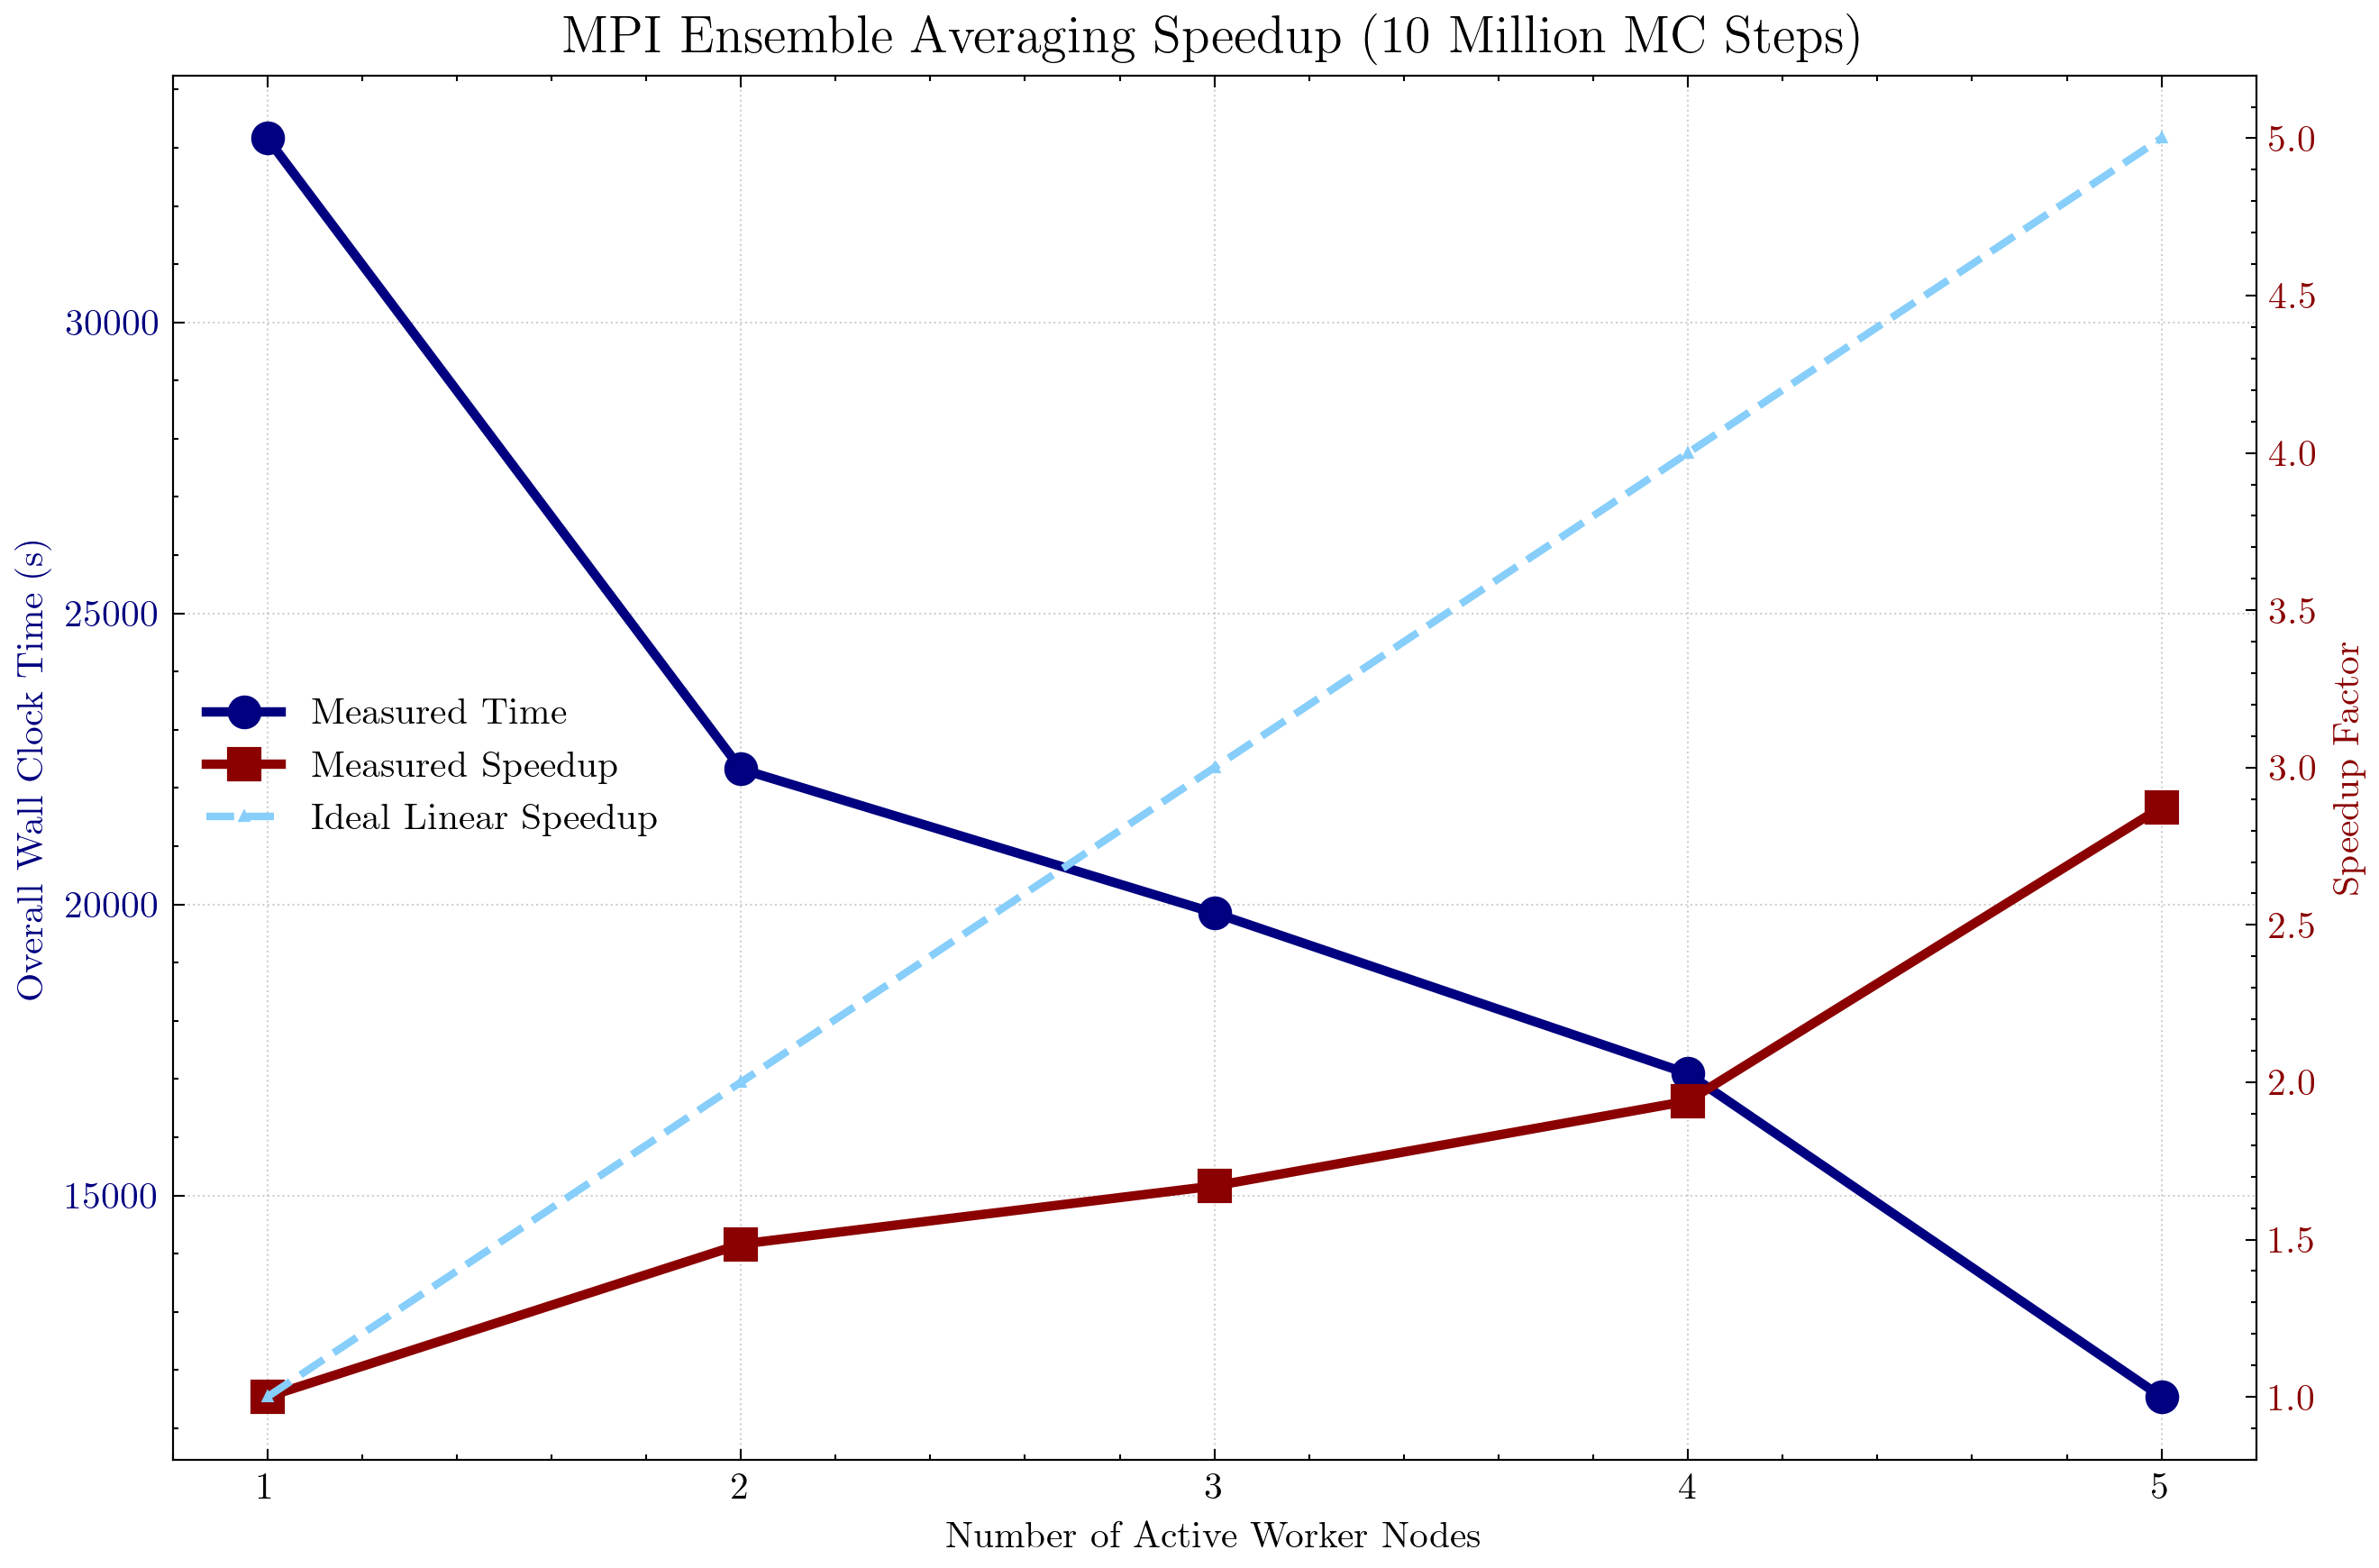
\includegraphics[keepaspectratio,alt={MPI Parallel Speedup Analysis}]{img/parallel_star_speedup_plot.png}}
\emph{Fig. x: Comparing timing \& efficiency of Ensemble Averaging with
various core count to Serial production run}

Simply adding more cores does not result in a perfectly linear speedup.
This can be attributed to parallelization overhead plus device hardware
bottlenecks. The most efficient use of cores is found in factors of 10
(2 \& 5 cores), in which cases all worker nodes are participating in the
final group of remaining 1M MCS steps. The non-factors of 10 could see
performance improvements with the addition of a dynamic algorithm that
determines how many steps are left once there are fewer 1M MCS jobs
remaining than cores participating. This would eliminates worker
``dead-time'' towards the end of the production run.

\subsection{Parallel Simulation
Results}\label{parallel-simulation-results}

\pandocbounded{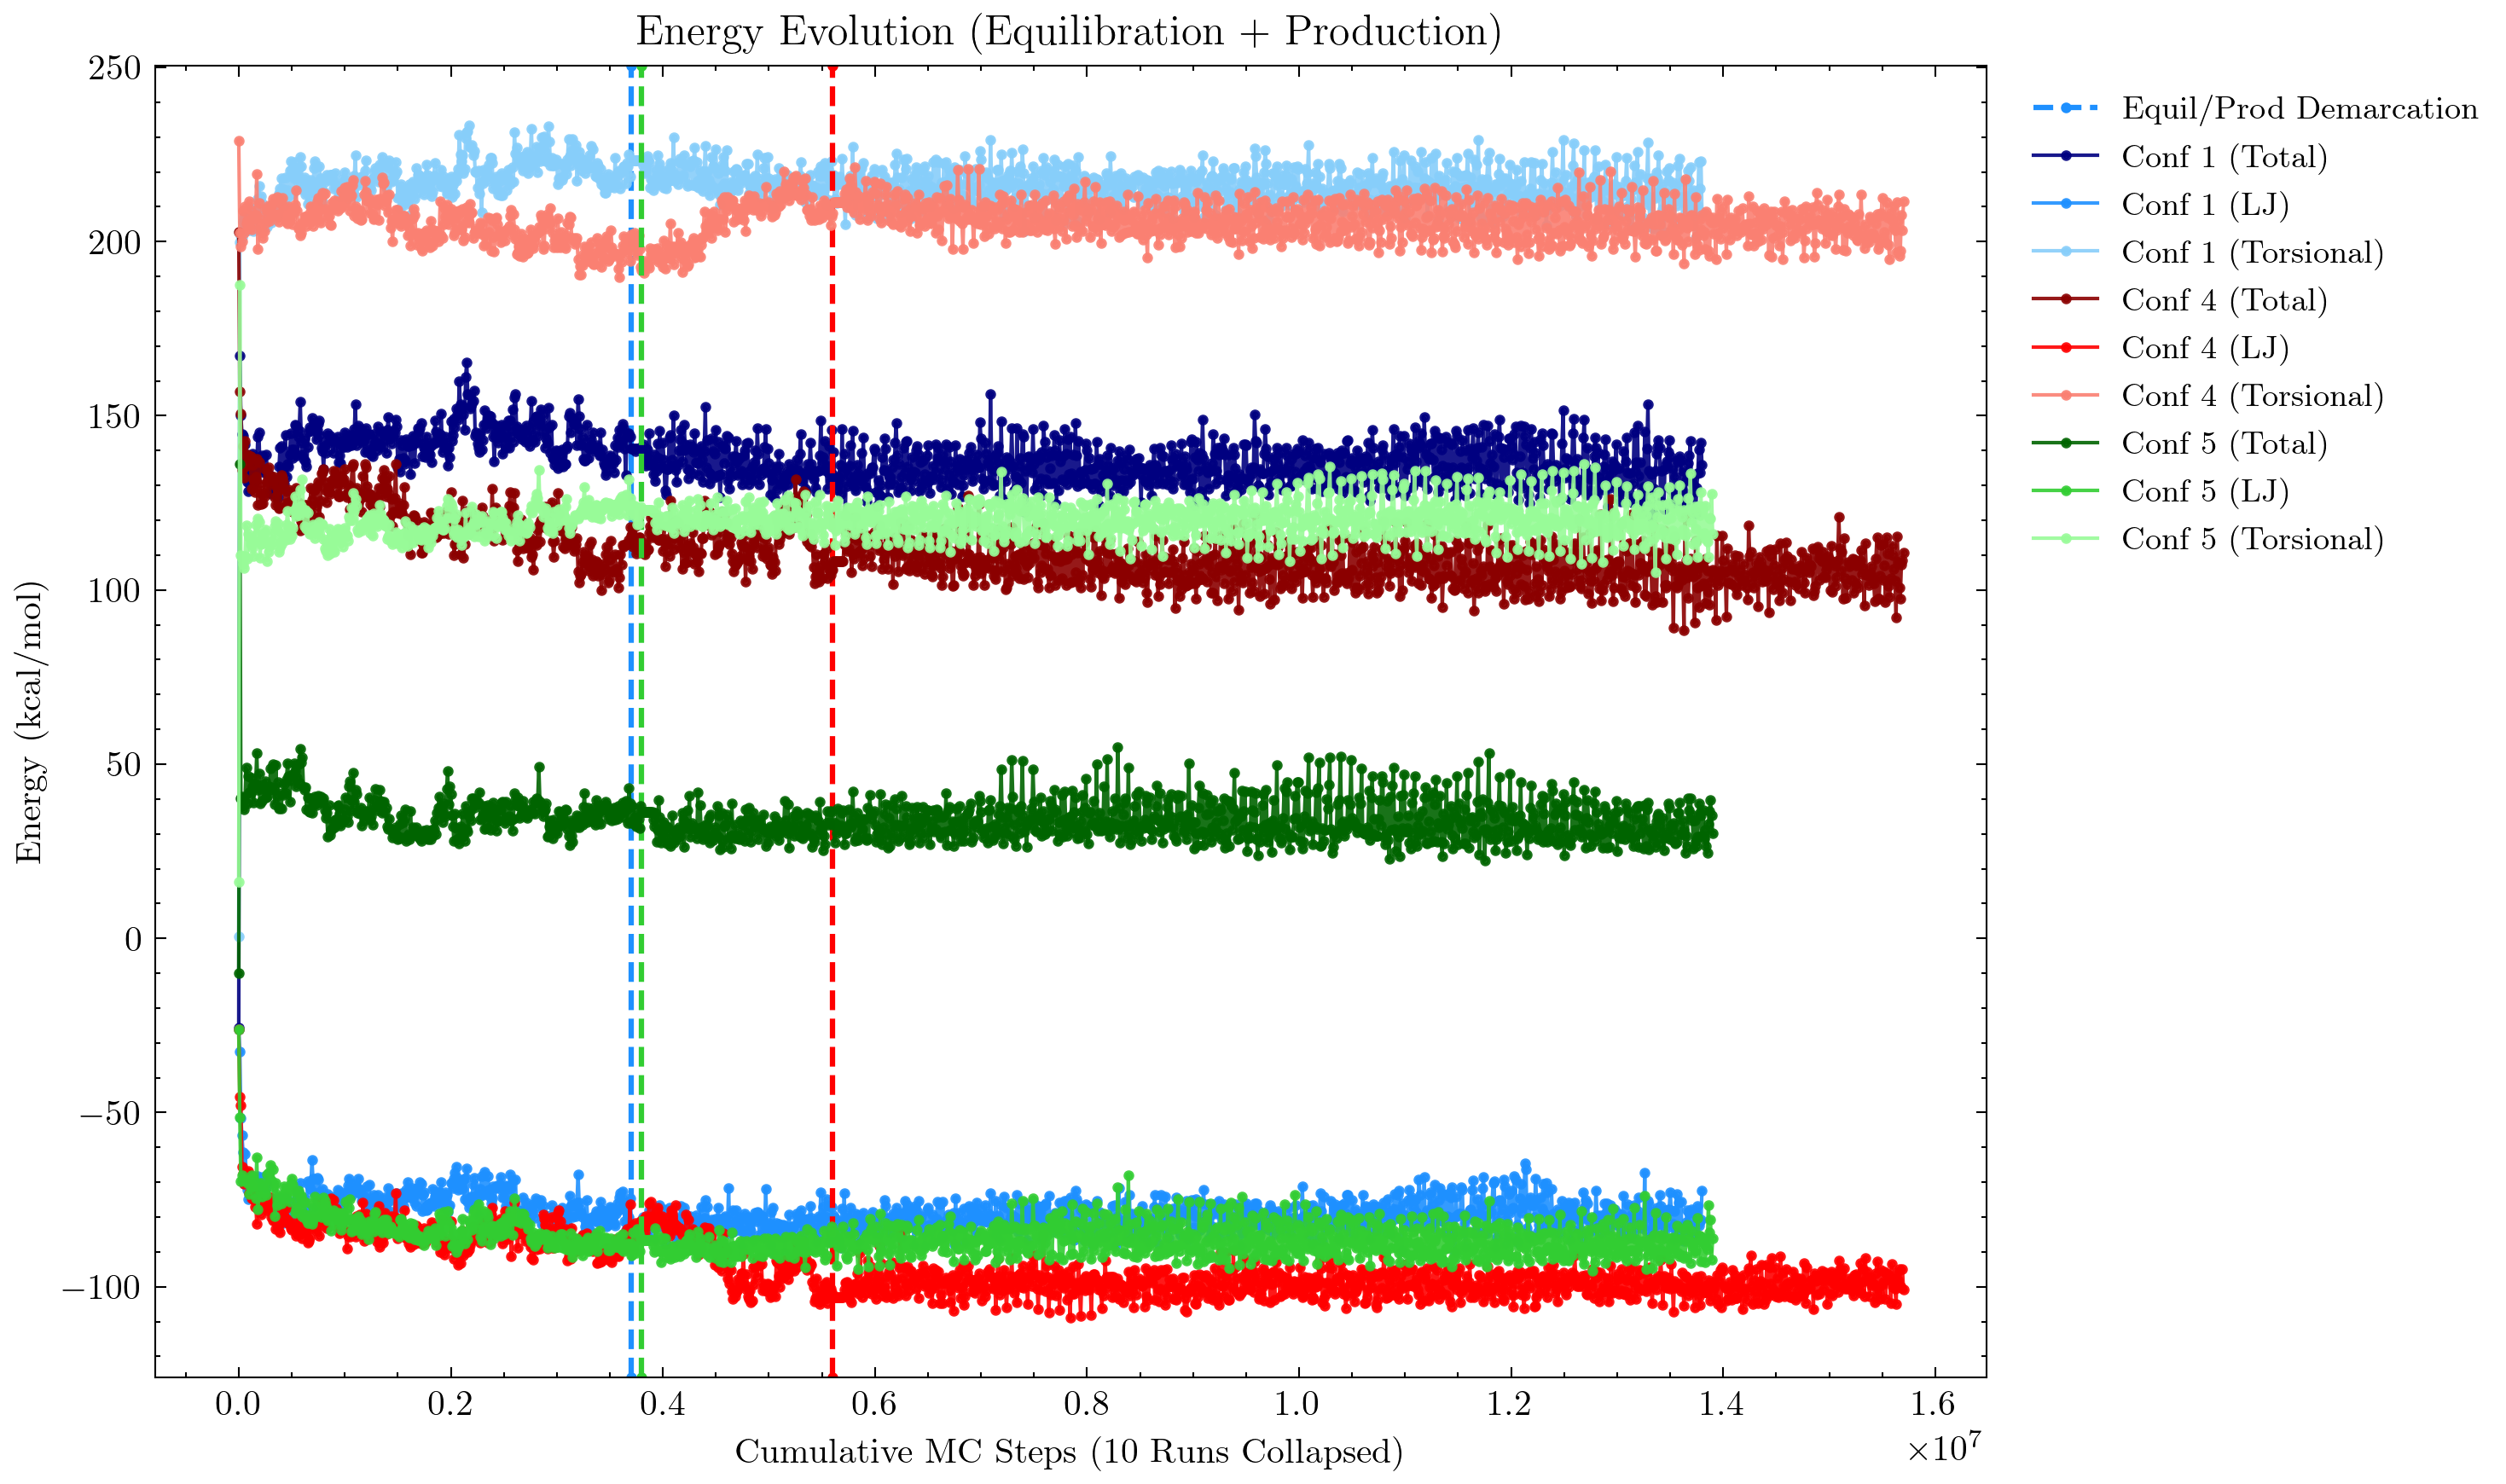
\includegraphics[keepaspectratio,alt={Energy Evolution}]{img/parallel_combined/parallel_energy_evolution.png}}
\emph{Fig. x: Total, LJ, \& Torsional Energy plots across various
initial conformations}

This plot tracks the total, Lennard-Jones (LJ), and torsional energy
trends over the progression of Monte Carlo Steps (MCS) for
configurations 1, 4, and 5. The vertical dashed lines mark the
transition point between equilibration and the subsequent 10-million
step production data.

In this particular instance of the combined simulation, the torsional
and LJ energy took longer to stabilize in configuration 4 than the other
configurations (1 \& 5), meaning equilibration took longer to pass the
Geweke equilibration determination test as indicated in the red,
vertical, dashed line. For this reason its combined simultion to run for
\(\sim1.55x10^7\) total steps.

An important observation and detail obtained from this graph is how
initial configuration influences the total energy within the simulation.
Configurations 1 \& 4 are rigid and straight helical structures,
respectively, while introducing random, out-of-plane tilts to
configuration 5 allowed it to find a much lower equilibrated torsional
(and therefore, total) energy.

\pandocbounded{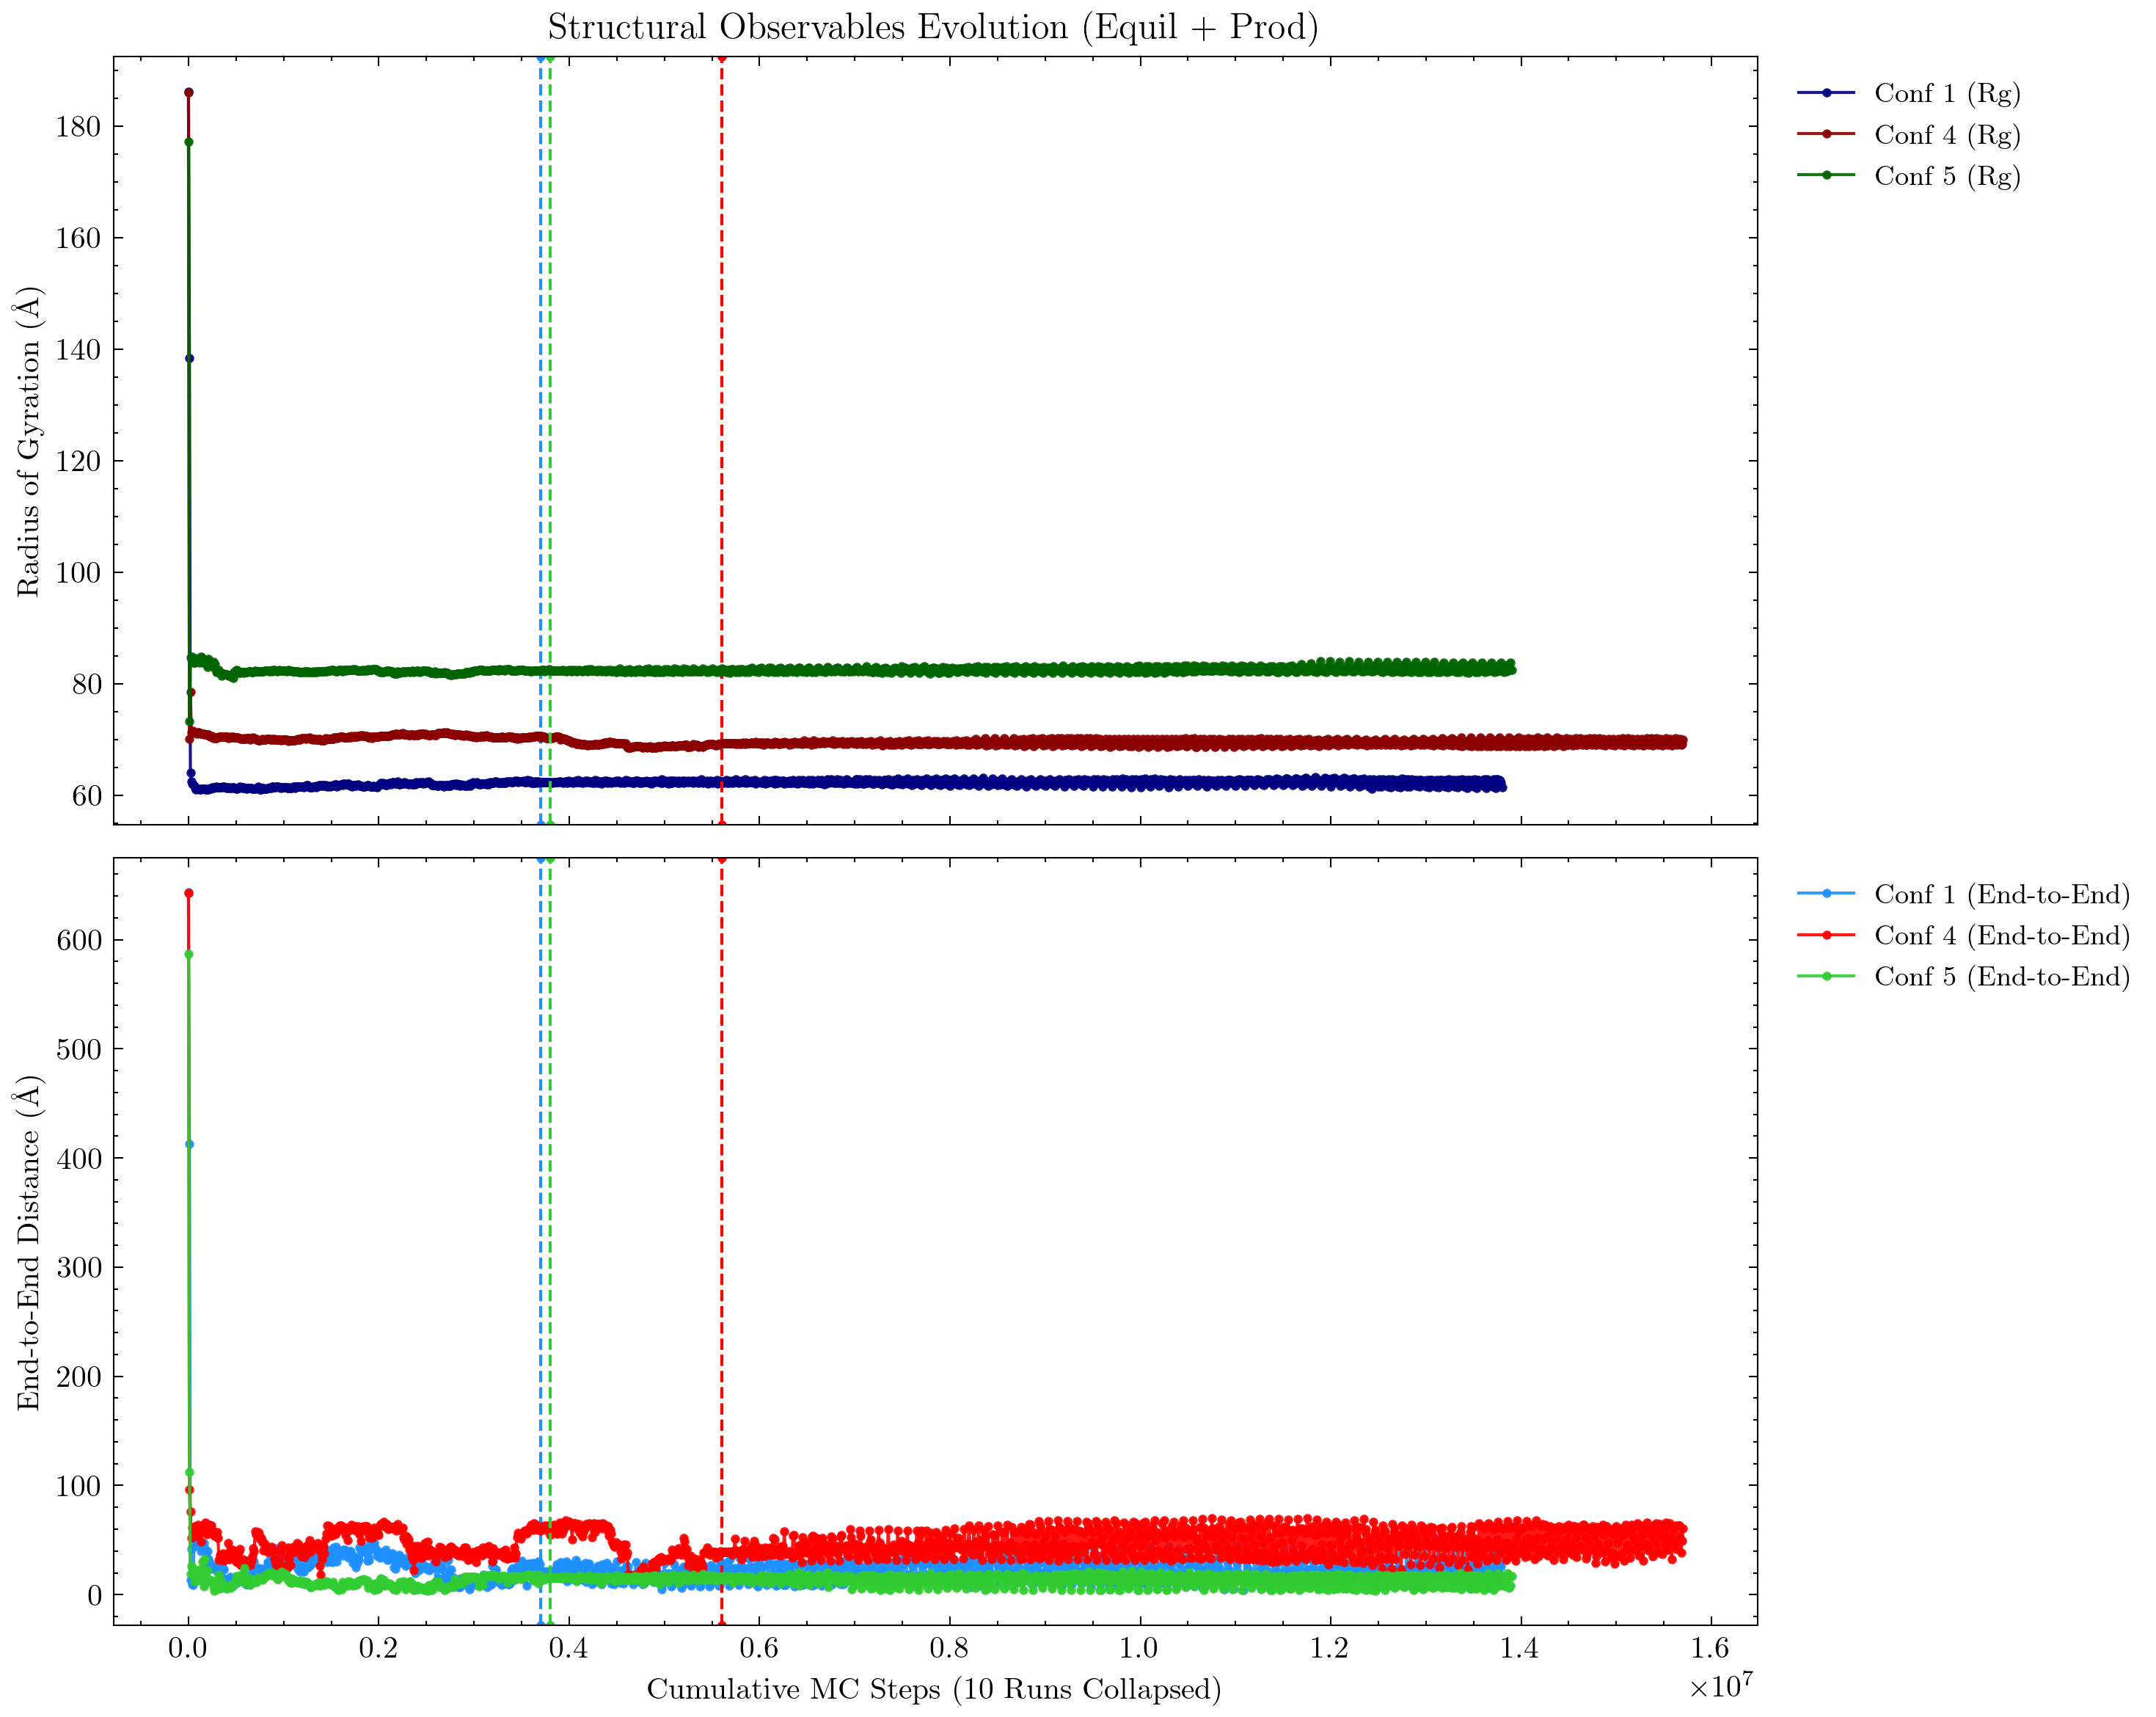
\includegraphics[keepaspectratio,alt={Energy Evolution}]{img/parallel_combined/parallel_observables_evolution.png}}
\emph{Fig. x: Radius of Gyration \& End-to-End Distance plots across
various initial conformations}

This chart displays the Radius of Gyration (Rg) and End-to-End Distance
for the different configurations. As with the energy plots above which
showed similar torsional energies between Conf 1 \& 4 while Conf 5 was
much lower after equilibration, the Rg for Conf 5 is the most distinct
here as well. Configuration 5, due to its initial out-of-plane tilts,
was able to better relax its bonds into low-energy rotational valleys,
allowing the chain to naturally untangle and adopt an expanded, looser
geometry, mathematically resulting in a higher Radius of Gyration.

\pandocbounded{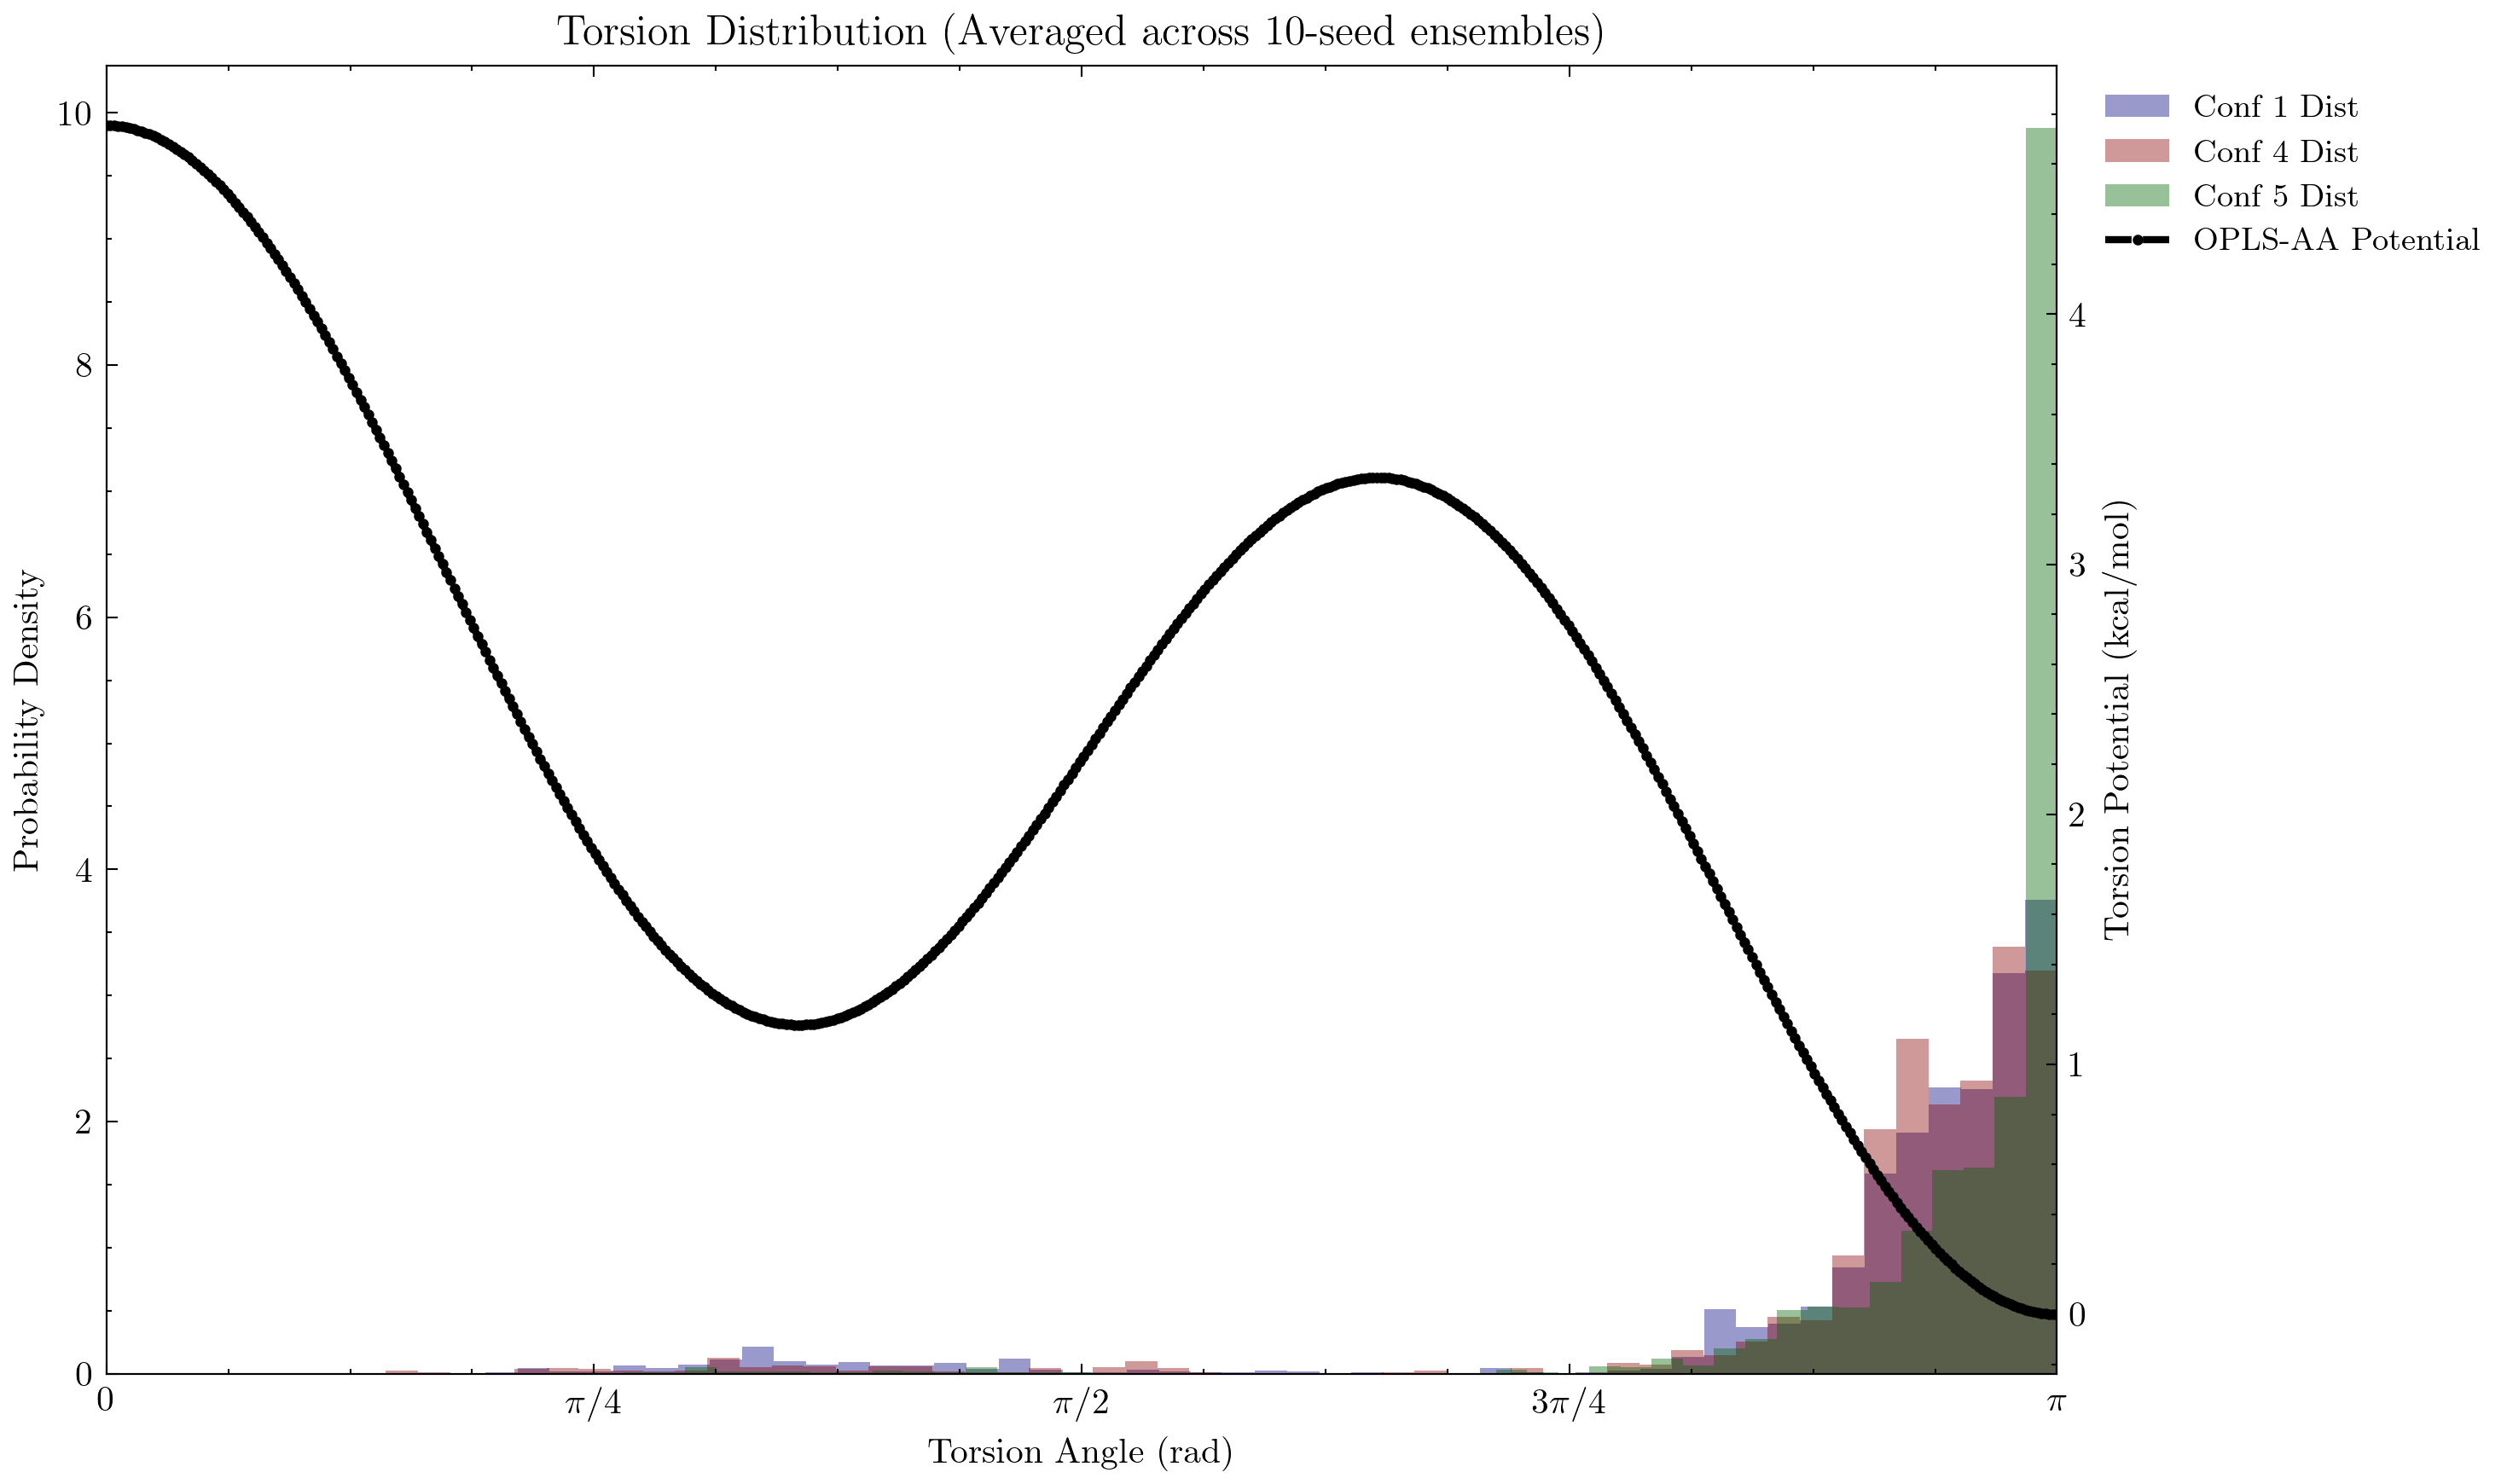
\includegraphics[keepaspectratio,alt={Energy Evolution}]{img/parallel_combined/parallel_torsion_distribution.png}}
\emph{Fig. x: Torsional distribution of post-equilibrated MCS across
various initial conformations}

The low-energy rotational valley relaxation tendency for Conf 5 is even
more apparent in this graph, which shows the probability density of the
each polymer exploring various dihedral (torsion) angles. Each
configuration's post-equilibration data is compared to the OPLS-AA
potential, where the results confirm the highest probability at \(\pi\)
(trans) configuration. While all configurations follow the expected
potential, Conf 5 adheres most closely, fully affirming the above energy
and observable data. Also of note is how the graph demonstrates the
expected rise in probablity around the potential's local minima at
\(\sim \pi/3\).

\subsection{UNUSED WRITING}\label{unused-writing}

\textbf{Project Impact}: While raw energy can sometimes settle rapidly,
physical tangles and extensions inside long macroscopic polymers often
require extended periods to fully untangle. The eventual flattening of
Rg and End-to-End values verifies that the polymer has achieved a true
spatial equilibrium. Furthermore, the steady stability throughout the
interleaved 10-million-step stretches proves that our technique of
batching multiple independent random-seeded 1-million-step parallel runs
generates completely robust, reliable macroscopic samples capable of
replacing a single sequential run.

\textbf{Graph Analysis}: This distribution visualizes the probability
density of the polymer exploring various dihedral (torsion) angles,
constructed exclusively by aggregating the pure post-equilibration
production data from the parallel worker nodes. It is superimposed over
the theoretical mathematical potential (dashed black line).

\textbf{Project Impact}: The histogram peaks for all three independent
polymer configurations perfectly align within the low-energy target
``valleys'' of the theoretical potential curve. This represents the
ultimate verification of our parallel approach. It definitively proves
that the Master-Worker topology's localized Metropolis acceptance
criteria functioned flawlessly across distributed nodes, accurately
guiding the simulated chains into realistic physical states. By
successfully distributing the load, we achieve massive speedups while
retaining the absolute energetic fidelity required for complex
structural modeling.
